A computation graph for a task parallel program is a directed acyclic graph that represents the execution of the program. The graph consists of nodes that denote the various parallel operations. The nodes also store references to the memory locations accessed by the tasks.

\begin{definition}
\textbf{Computation Graph:} A Computation Graph 
$G = \tuple{N, E, \delta, \omega}$ of a task parallel program \textbf{P} with input $\psi$ is a directed acyclic graph where

\begin{itemize}
\item $N$ is a finite set of nodes
\item $E \subseteq N \times N$ is a set of directed edges. 
\item $\delta$ is the function that maps $N$ to the unique identifiers for the shared locations read by the tasks.
\begin{center}
$\delta : (N \mapsto 2^{V})$ 
\end{center}
\item $\omega$ is the function that maps $N$ to the unique identifiers for the shared locations written by the tasks.
\begin{center}
$\omega : (N \mapsto 2^{V})$ 
\end{center}
\end{itemize}
where V is the set of the unique identifiers for the shared locations.
\end{definition}

\begin{figure}
  \centering
        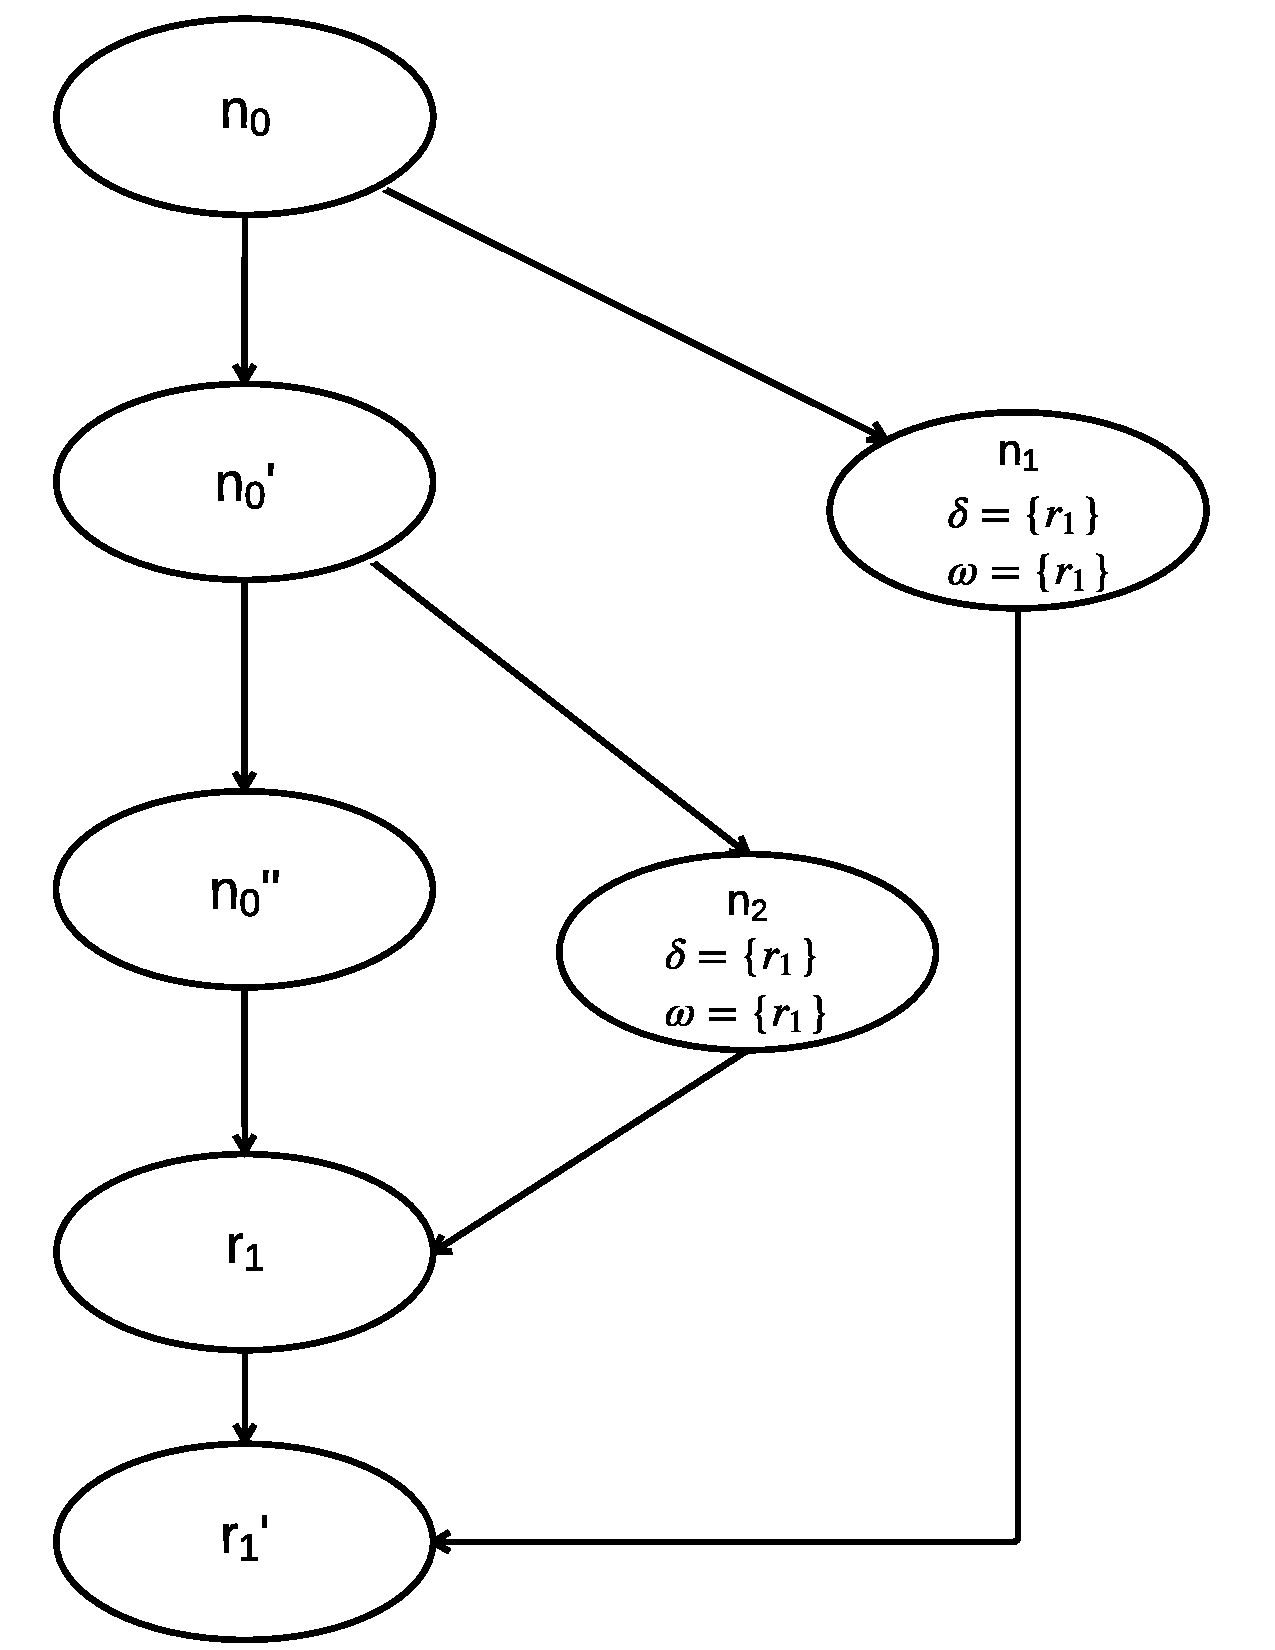
\includegraphics[width=0.5\textwidth]{../figs/Fig3-1.pdf}
    \caption{Computation Graph Example.}
    \label{fig:cg}
\end{figure}

\figref{fig:cg} shows a sample computation graph. In this graph, nodes $n_0$, $n_0'$, $n_0''$, $r_1$, and $r_1'$ belong to task $t_0$. Task $t_0$ spawns two tasks $t_1$ and $t_2$. Node $n_1$ belongs to task $t_1$ and node $n_2$ belongs to task $t_2$. Node $r_1$ and $r_1'$ are join nodes for tasks $t_1$ and $t_2$. 

\begin{algorithm}
\caption{Data Race detection in a computation graph.} \label{algo:drd}
\begin{algorithmic}[1]
\Function{DetectRace}{$Computation Graph \ G$}\label{loc:topo}
\State N := Topologically ordered nodes in G
\For {i in [1, $|N|$]}
\State $n = N[i]$
\For {j in [i+1, $|N|$]} 
\State $n' = N[j]$
\If {$ (n \nprec n') \land (n' \nprec n)$}  \label{loc:path} \label{loc:forall}
	\State \textbf{bool} $\mathtt{rw} = (\delta(n) \cap \omega(n') \neq \emptyset) $
	\State \textbf{bool} $\mathtt{wr} = (\omega(n) \cap \delta(n') \neq \emptyset) $
	\State \textbf{bool} $\mathtt{ww} = (\omega(n) \cap \omega(n') \neq \emptyset)$
		\If {$( \mathtt{rw} \lor \mathtt{wr}  \lor \mathtt{ww} )$} \label{loc:intersection}
			\State \textbf{Report Data Race and Exit} \label{loc:datarace}
		\EndIf
\EndIf
 \EndFor
 \EndFor
\EndFunction  
\end{algorithmic}
\end{algorithm}

Computation graphs can be used to detect data races in parallel programs. Every node in the computation graph represents a block of sequential operations. A computation graph is a partially ordered set of nodes that gives the relationship of the tasks in the program. The transitive closure of the graph gives the reachability of the nodes. The order between any two nodes $n_1$ and $n_2$ is given as $n_1 \prec n_2$, meaning that $n_1$ happens before $n_2$. The operations that may execute in parallel are unordered: $n_1 \nprec n_2$ and $n_2 \nprec n_1$, i. e. $n_1$ does not happen before $n_2$ and $n_2$ does not happen before $n_1$. Once these unordered nodes are identified, the memory accessed by the operations performed in these nodes is checked to detect data races. 

Algorithm \ref{algo:drd} gives the pseudo-code of the algorithm to detect data races in computation graphs. It takes the computation graph as input and reports a data race if an access violation is observed in the graph. The algorithm works as follows. The nodes in the computation graph are added to a topologically sorted set on \lineref{loc:topo}. The $i^{th}$ node in the order is given by N[i]. The nodes are traversed in order and each node is compared to every node that comes later in the topological ordering. \lineref{loc:path} checks if the nodes $n$ and $n'$ are  unordered. If the nodes are unordered, then the sets of memory locations accessed by each node are checked for conflict on \lineref{loc:intersection}. If any of the sets shares an element, then any one of those elements is a location where a data race occurs in the program. A data race is reported by the algorithm on \lineref{loc:datarace}. If the intersecting sets are empty, then the algorithm proceeds to check the next node until either a data race is reported or all the nodes have been verified.

Consider again the example in \figref{fig:cg} with the topological ordering: $n_0$, $n_0'$, $n_0''$, $n_1$, $r_1$, $n_2$, and $r_1'$. Node $n_0$ happens before all other nodes so it cannot data race with anything. The next node in the topological ordering is $n_0'$. It is not ordered relative to $n_1$ so $n_0^\prime$ and $n_1$ are parallel. No race is reported and the analysis proceeds because there are no conflicting accesses made by these nodes. All the nodes are checked one by one in a similar way. The nodes $n_1$ and $n_2$ are unordered since there is no path from $n_1$ to $n_2$ and both are writing to variable $r_1$. Therefore, $\mathtt{ww}$ is set to true and a race is reported for these two nodes on $r_1$.

The algorithm runs in quadratic time for the number of nodes in the computation graph. The topological ordering of nodes can be done in $\mathcal{O}$(N$^2$). When nodes are topologically ordered, reachability of nodes can be checked in $\mathcal{O}$(N) time. Therefore, the time required to check if two nodes are executing in parallel is $\mathcal{O}$(N$^2$). The time required to check the intersection of read or write sets of shared locations is $\mathcal{O}$($m_1 +  m_2$) where $m_1$ and $m_2$ are the sizes of the two sets. ($m_1 + m_2$) is much smaller than N. Therefore, the time complexity of Algorithm \ref{algo:drd}  is $\mathcal{O}$(N$^2$).

\begin{definition} 
\textbf{Sound:} A data race detection algorithm is sound if it does not miss any data race in a program for a given input.
\end{definition}

If the sound algorithm declares a program to be data race free, no race can exist in execution of the program for the given input on any schedule; although, it may reject programs as having data races when in fact they do not. It may under-approximate the set of data race free programs.

\begin{definition}
\textbf{Complete}:  A data race detection algorithm is complete if it does not report data races in programs that are data race free.
\end{definition}

A complete algorithm may accept programs as data race free when in fact they have data races. It may over-approximate the set of data race free programs.

\begin{theorem} \label{thm:graph}
Algorithm \ref{algo:drd} is sound and complete for a given a computation graph $G$.
\end{theorem}

\begin{proof}
The computation graph is a directed acyclic graph. The transitive closure of the graph gives the reachibility relationship of the tasks. The transitive closure is a strict partial order over the nodes of the graph. The data race detection algorithm checks if nodes $n$ and $n^\prime$ in the graph are unordered on Line \ref{loc:forall}. The statements may be executed in parallel by these nodes. The memory accessed by these tasks is compared and a race is reported if a conflict is detected on Line \ref{loc:datarace}. Therefore, when algorithm \ref{algo:drd} declares a computation graph to be data race free, no race can exist in that graph and when a race is reported by the algorithm, there definitely exists two tasks that execute in parallel and have conflicting accesses to a shared variable. Hence, Algorithm \ref{algo:drd} is sound and complete for a given computation graph.
\end{proof}
